\hideheader
\section{Διδασκαλία αλγορίθμων}

Η διδασκαλία των αλγορίθμων αποτελεί μία από τις πιο κρίσιμες πτυχές της εκπαίδευσης στην πληροφορική και στις επιστήμες των υπολογιστών. Η κατανόηση και η εφαρμογή των αλγορίθμων είναι θεμελιώδεις δεξιότητες που πρέπει να αποκτήσουν οι μαθητές για να επιτύχουν στην επίλυση προβλημάτων και στον προγραμματισμό. Σε αυτό το κεφάλαιο, θα εξεταστούν οι βασικές θεωρητικές αρχές της διδασκαλίας αλγορίθμων, οι διάφορες μεθοδολογίες που έχουν αναπτυχθεί για αυτόν τον σκοπό, καθώς και οι τεχνολογίες που μπορούν να ενσωματωθούν για τη βελτίωση της μαθησιακής εμπειρίας.

\subsection{Θεωρητικά θεμέλια της διδασκαλίας αλγορίθμων}

Η επίλυση προβλημάτων είναι κεντρική στη διδασκαλία των αλγορίθμων. Οι Polya και Hayes έχουν προτείνει ότι η διαδικασία επίλυσης προβλημάτων περιλαμβάνει τέσσερα κύρια στάδια: την κατανόηση του προβλήματος, τον σχεδιασμό ενός πλάνου, την εφαρμογή του πλάνου και την ανασκόπηση του αποτελέ-σματος\cite{bodner_role_1987,crepinsek_note_2012}. Αυτά τα στάδια μπορούν να βοηθήσουν τους μαθητές να αναπτύξουν μια συστηματική προσέγγιση στην επίλυση προβλημάτων και να κατανοήσουν βαθύτερα τη λογική πίσω από τους αλγορίθμους.

Οι αλγόριθμοι ορίζονται ως \("\)κανόνες για τον υπολογισμό κάτι, ειδικά από μη-χανές\("\) και μπορούν να ακολουθηθούν σχεδόν αυτόματα από συστήματα όπως οι υπολογιστές\cite{bodner_role_1987}. Η διδασκαλία των αλγορίθμων απαιτεί την κατανόηση αυτών των κανόνων και την εφαρμογή τους σε διάφορα προβλήματα, από απλές μαθηματικές πράξεις έως πολύπλοκα προγραμματιστικά προβλήματα.

% ========================================

\subsection{Μέθοδοι διδασκαλίας αλγορίθμων}

Η διδασκαλία των αλγορίθμων μπορεί να προσεγγιστεί μέσω διαφόρων μεθόδων, κάθε μία από τις οποίες προσφέρει συγκεκριμένα πλεονεκτήματα και προκλήσεις.

\subsubsection{Παραδοσιακή διδασκαλία}

Η παραδοσιακή διδασκαλία περιλαμβάνει τη χρήση διαλέξεων και βιβλίων ως κύρια μέσα για τη διδασκαλία των βασικών εννοιών και τεχνικών των αλγορίθμων. Σε αυτή τη μέθοδο, οι εκπαιδευτικοί παρουσιάζουν το υλικό μέσα από διαλέξεις και οι μαθητές ενθαρρύνονται να διαβάζουν τα σχετικά βιβλία για να κατανοήσουν τις θεωρητικές έννοιες. Παρόλο που αυτή η μέθοδος είναι αποτελεσματική για την παράδοση μεγάλου όγκου πληροφορίας και την παρουσίαση των θεωρητικών θεμελίων, συχνά δεν παρέχει αρκετή διαδραστικότητα και πρακτική εφαρμογή, που είναι απαραίτητα για την πλήρη κατανόηση των αλγορίθμων\cite{__2017}.

\subsubsection{Μάθηση βασισμένη σε παραδείγματα}

Η μάθηση βασισμένη σε παραδείγματα επικεντρώνεται στη χρήση παραδειγμάτων και ασκήσεων για τη διδασκαλία των αλγορίθμων. Σε αυτή τη μέθοδο, οι μαθητές διδάσκονται μέσω της παρουσίασης συγκεκριμένων παραδειγμάτων που δείχνουν την πρακτική εφαρμογή των αλγορίθμων. Τα παραδείγματα βοηθούν τους μαθητές να κατανοήσουν πώς να εφαρμόζουν τους αλγορίθμους σε πραγματικά προβλήματα και να αναπτύξουν δεξιότητες επίλυσης προβλημάτων. Αυτή η μέθοδος είναι ιδιαίτερα αποτελεσματική για τη διευκρίνιση σύνθετων εννοιών και την ενίσχυση της πρακτικής κατανόησης\cite{crepinsek_note_2012}.

Τα παραδείγματα αυτά πολλές φορές μπορούν να έχουν τη μορφή εκπαιδευτικών λογισμικών ή βίντεο. Τα εκπαιδευτικά λογισμικά προσφέρουν διαδραστικές ασκήσεις και παραδείγματα που βοηθούν τους μαθητές να κατανοήσουν τις βασικές αρχές των αλγορίθμων. Αυτά τα λογισμικά συχνά περιλαμβάνουν εργαλεία για την οπτικοποίηση των αλγορίθμων, επιτρέποντας στους μαθητές να βλέπουν βήμα προς βήμα την εκτέλεση του αλγορίθμου και να κατανοούν καλύτερα την εσωτερική λειτουργία του\cite{__2017}. Τα μαθήματα με βίντεο παρέχουν μια οπτική και ακουστική προσέγγιση στη διδασκαλία των αλγορίθμων. Αυτή η μέθοδος μπορεί να είναι ιδιαίτερα αποτελεσματική για την επεξήγηση σύνθετων εννοιών και την παροχή παραδειγμάτων βήμα προς βήμα. Τα βίντεο επιτρέπουν στους μαθητές να παρακολουθούν την επίλυση προβλημάτων σε πραγματικό χρόνο και να επαναλαμβάνουν τα βήματα όποτε χρειάζεται\cite{__2022}.

Υπάρχουν διάφορα λογισμικά τα οποία προσομοιώνουν αλγόριθμους. Μερικά από αυτά είναι:
\begin{itemize}
    \item \textbf{VisuAlgo\cite{noauthor_visualising_nodate}:} Προσομοιώνει αλγόριθμους επιτρέποντας στον χρήστη να δει κάθε βήμα που ακολουθεί ο αλγόριθμος.

    \begin{figure}[H]
        \centering
        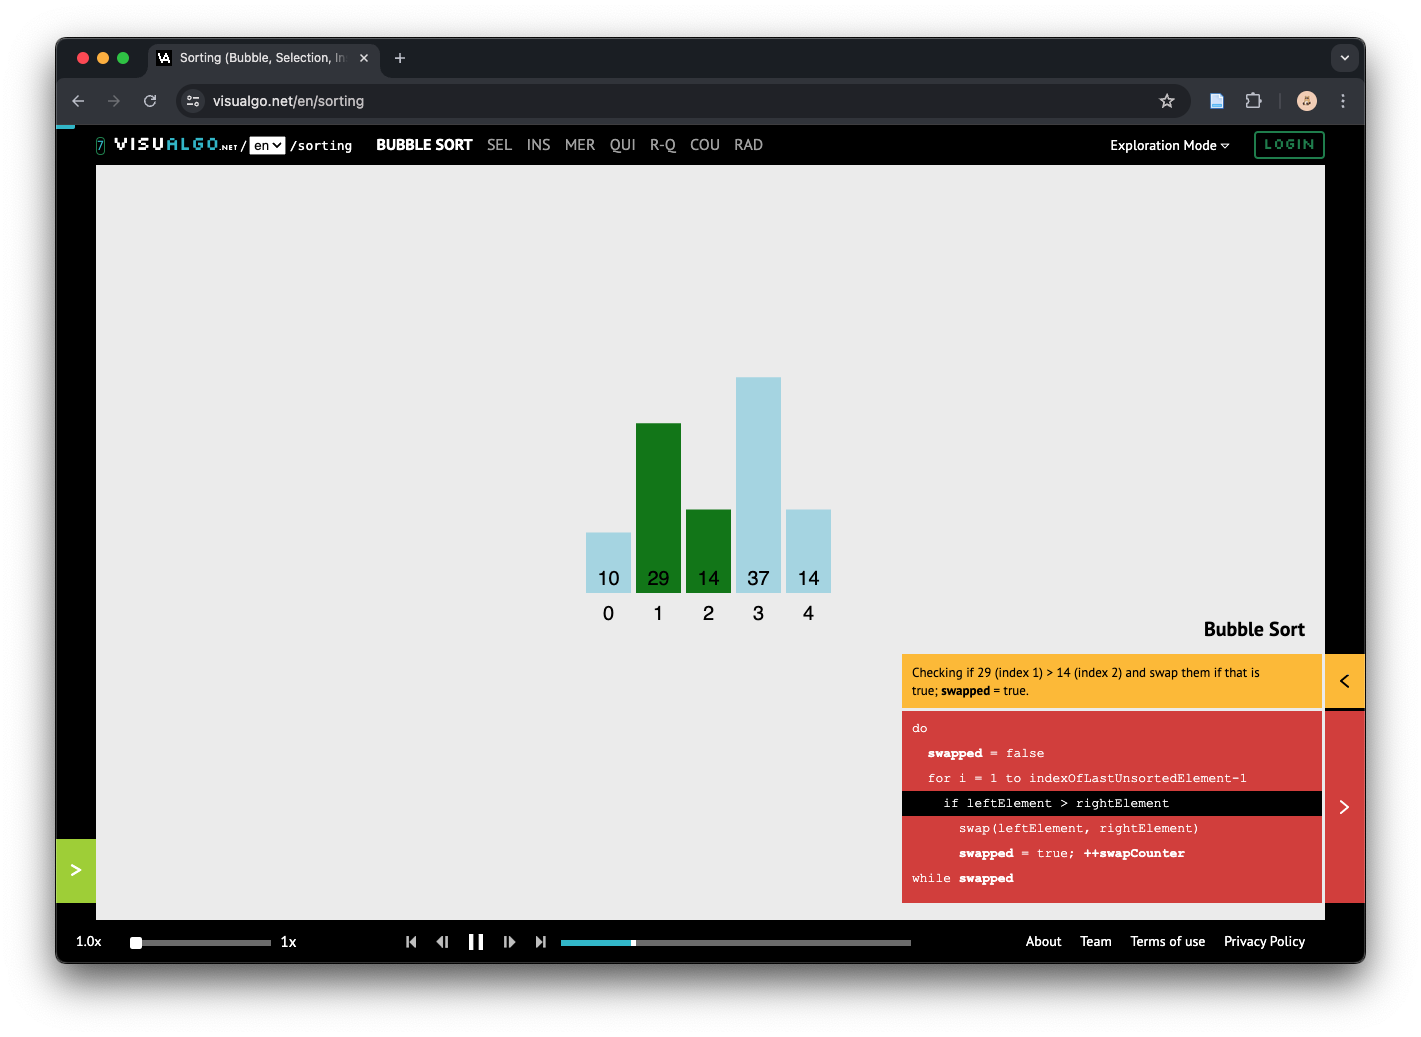
\includegraphics[width=0.8\linewidth]{sections/2/images/visualgo}
        \caption{Παράδειγμα προσομοίωσης αλγορίθμου στο VisuAlgo}
        \label{fig:visualgo}
    \end{figure}
    
    \item \textbf{Sort Visualizer\cite{noauthor_sort_nodate}:} Προσφέρει ποικιλία αλγορίθμων και επιτρέπει την προσομοίωση με μεγάλο αριθμό τιμών για οπτικοποίηση του χρόνου που χρειάζεται κάθε αλγόριθμος να ολοκληρωθεί.

    \begin{figure}[H]
        \centering
        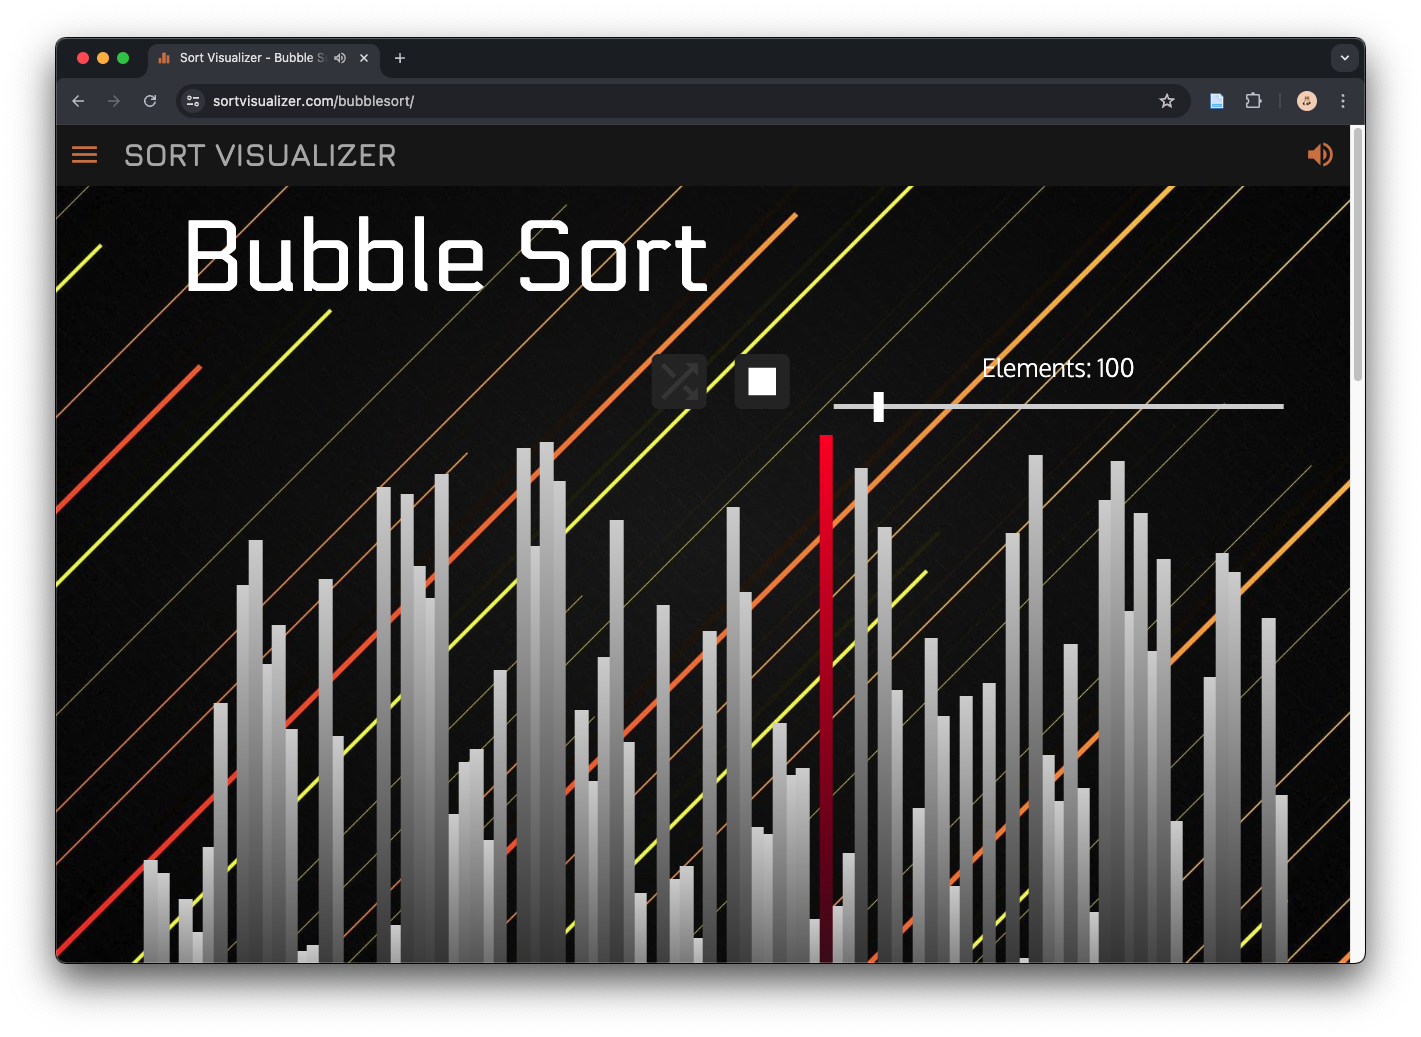
\includegraphics[width=0.8\linewidth]{sections/2/images/sort_visualizer}
        \caption{Παράδειγμα προσομοίωσης αλγορίθμου στο Sort Visualizer}
        \label{fig:sort_visualizer}
    \end{figure}
\end{itemize}

\subsubsection{Διδασκαλία μέσω έργων}

Η διδασκαλία μέσω έργων περιλαμβάνει την ανάθεση έργων στους μαθητές, τα οποία απαιτούν την εφαρμογή αλγορίθμων για την επίλυση συγκεκριμένων προβλημάτων. Αυτή η προσέγγιση ενθαρρύνει την ενεργή μάθηση και την ανάπτυξη πρακτικών δεξιοτήτων προγραμματισμού. Οι μαθητές καλούνται να εργαστούν σε πραγματικά προβλήματα, χρησιμοποιώντας τους αλγορίθμους που έχουν μάθει, και να αναπτύξουν λύσεις. Η μέθοδος αυτή προωθεί την κριτική σκέψη, τη δημιουργικότητα και την ικανότητα εφαρμογής θεωρητικών γνώσεων σε πρακτικές καταστάσεις\cite{bodner_role_1987}.

Ένα παράδειγμα της διδασκαλίας μέσω έργου είναι η εκτέλεση βημάτων μιας διαδικασίας, με σκοπό τη δημιουργία μιας χειροτεχνίας. Οι μαθητές κατά τη διάρκεια της διαδικασίας δεν καταλαβαίνουν πως αυτό που εκτελούν πραγματικά είναι βήματα ενός αλγορίθμου, κάτι που έχει ως αποτέλεσμα την κατανόηση της λογικής σε βαθύ επίπεδο\cite{__2022}.

\begin{figure}[H]
    \centering
    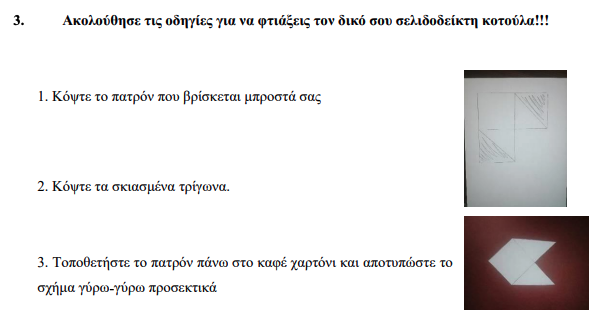
\includegraphics[width=0.8\linewidth]{sections/2/images/chicken}
    \caption{Διδασκαλία μέσω έργου με τη δημιουργία χειροτεχνίας}
    \label{fig:cicken}
\end{figure}

\subsubsection{Μάθηση μέσω συνεργασίας}

Η μάθηση μέσω συνεργασίας περιλαμβάνει την εργασία των μαθητών σε ομάδες για την επίλυση προβλημάτων αλγορίθμων. Αυτή η μέθοδος ενθαρρύνει τη συνεργασία και την επικοινωνία μεταξύ των μαθητών, επιτρέποντάς τους να μοιράζονται ιδέες και να μαθαίνουν από τις εμπειρίες των άλλων. Η συνεργατική μάθηση μπορεί να βελτιώσει την κατανόηση των αλγορίθμων, καθώς οι μαθητές μπορούν να συζητήσουν και να εξηγήσουν τις έννοιες μεταξύ τους, ενισχύοντας έτσι τη συνολική μάθηση\cite{crepinsek_note_2012}.

\subsubsection{Διαδραστική διδασκαλία}

Η διαδραστική διδασκαλία χρησιμοποιεί διαδραστικά εργαλεία και πλατφόρμες που επιτρέπουν στους μαθητές να πειραματιστούν με αλγορίθμους σε πραγματικό χρόνο. Αυτή η μέθοδος μπορεί να περιλαμβάνει τη χρήση εκπαιδευτικών παιχνιδιών, προσομοιώσεων και άλλων εργαλείων που κάνουν τη μάθηση πιο ελκυστική και αποδοτική. Οι μαθητές μπορούν να δοκιμάσουν διάφορες προσεγγίσεις, να δουν τα αποτελέσματα των ενεργειών τους και να αναπτύξουν μια βαθύτερη κατανόηση των αλγορίθμων μέσω της άμεσης αλληλεπίδρασης και του πειραματισμού\cite{__2022}.

Ένα από τα βασικότερα εργαλεία της διαδραστικής διδασκαλίας είναι οι προσομοιώσεις και τα παιχνίδια. Αυτά παρέχουν ένα διασκεδαστικό και διαδραστικό τρόπο για τη διδασκαλία των αλγορίθμων. Οι μαθητές μπορούν να πειραματιστούν με αλγορίθμους και να δουν τα αποτελέσματα των ενεργειών τους σε πραγματικό χρόνο. Οι προσομοιώσεις επιτρέπουν στους μαθητές να αναπτύξουν δεξιότητες επίλυσης προβλημάτων μέσω της πρακτικής εφαρμογής και της επανάληψης\cite{crepinsek_note_2012}.

Ένα παράδειγμα εκπαιδευτικού λογισμικού είναι το \("\)Παίζοντας με τους αλγόριθμους (Ταξινόμηση κι Αναζήτηση)\("\), το οποίο κατασκευάστηκε ως βοηθητικό υλικό για εμβάθυνση στους αλγορίθμους που διδάσκονται στο μάθημα της Ανάπτυξης σε Προγραμματιστικό Περιβάλλον της Τεχνολογικής Κατεύθυνσης της Γ’ Λυκείου\cite{__2017}.

\begin{figure}[H]
    \centering
    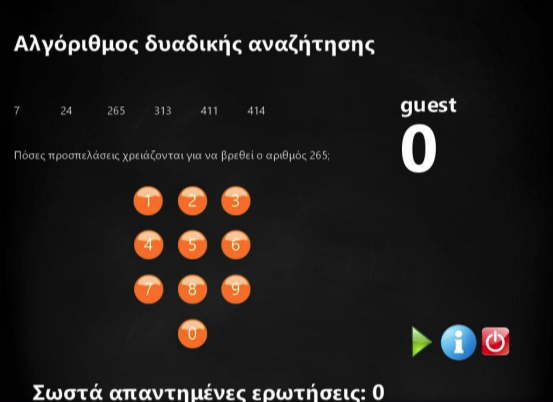
\includegraphics[width=0.8\linewidth]{sections/2/images/interactive}
    \caption{Διαδραστική διδασκαλία με εκπαιδευτικό λογισμικό}
    \label{fig:interactive}
\end{figure}

Όπως φαίνεται στην εικόνα \ref{fig:interactive}, ο εκπαιδευόμενος καλείται να βρει ένα στοιχείο κάθε φορά χρησιμοποιώντας τον αλγόριθμο δυαδικής αναζήτησης σε δέκα διαφορετικές περιπτώσεις, όπου οι πίνακες στοιχείων έχουν διαφορετικό μέγεθος κάθε φορά. Για κάθε σωστή απάντηση ο χρήστης κερδίζει δέκα βαθμούς, ενώ για κάθε λανθασμένη απάντηση χάνει πέντε. Επιπλέον, από το κάτω μέρος της οθόνης, ο χρήστης μπορεί να επιλέξει να δει τις οδηγίες χρήσης του παιχνιδιού\cite{__2017}.
